% ----------------------------------------------------------
\chapter{Desenvolvimento do Projeto}
% ----------------------------------------------------------

Depois das definições apresentadas e da escolha de componentes apresentada na seção anterior, foi possível construir um esquemático elétrico, que esquematiza a PCB do OBDH. Nesse capítulo, discutir-se-á circuitos específicos mais relevantes do projeto, usando o esquemático pronto, que se encontra no Anexo I.

\section{Conversores de Potência}

Partindo do princípio que o módulo EPS da terceira geração de módulos do SpaceLab será capaz de fornecer 3,3 V para o OBDH, foi proposta uma cascata de potência descrita na Figura \ref{fig:power}. Nela, são suprimidos os circuitos de proteção que serão descritos posteriormente.

\begin{figure}[H]
    \centering
    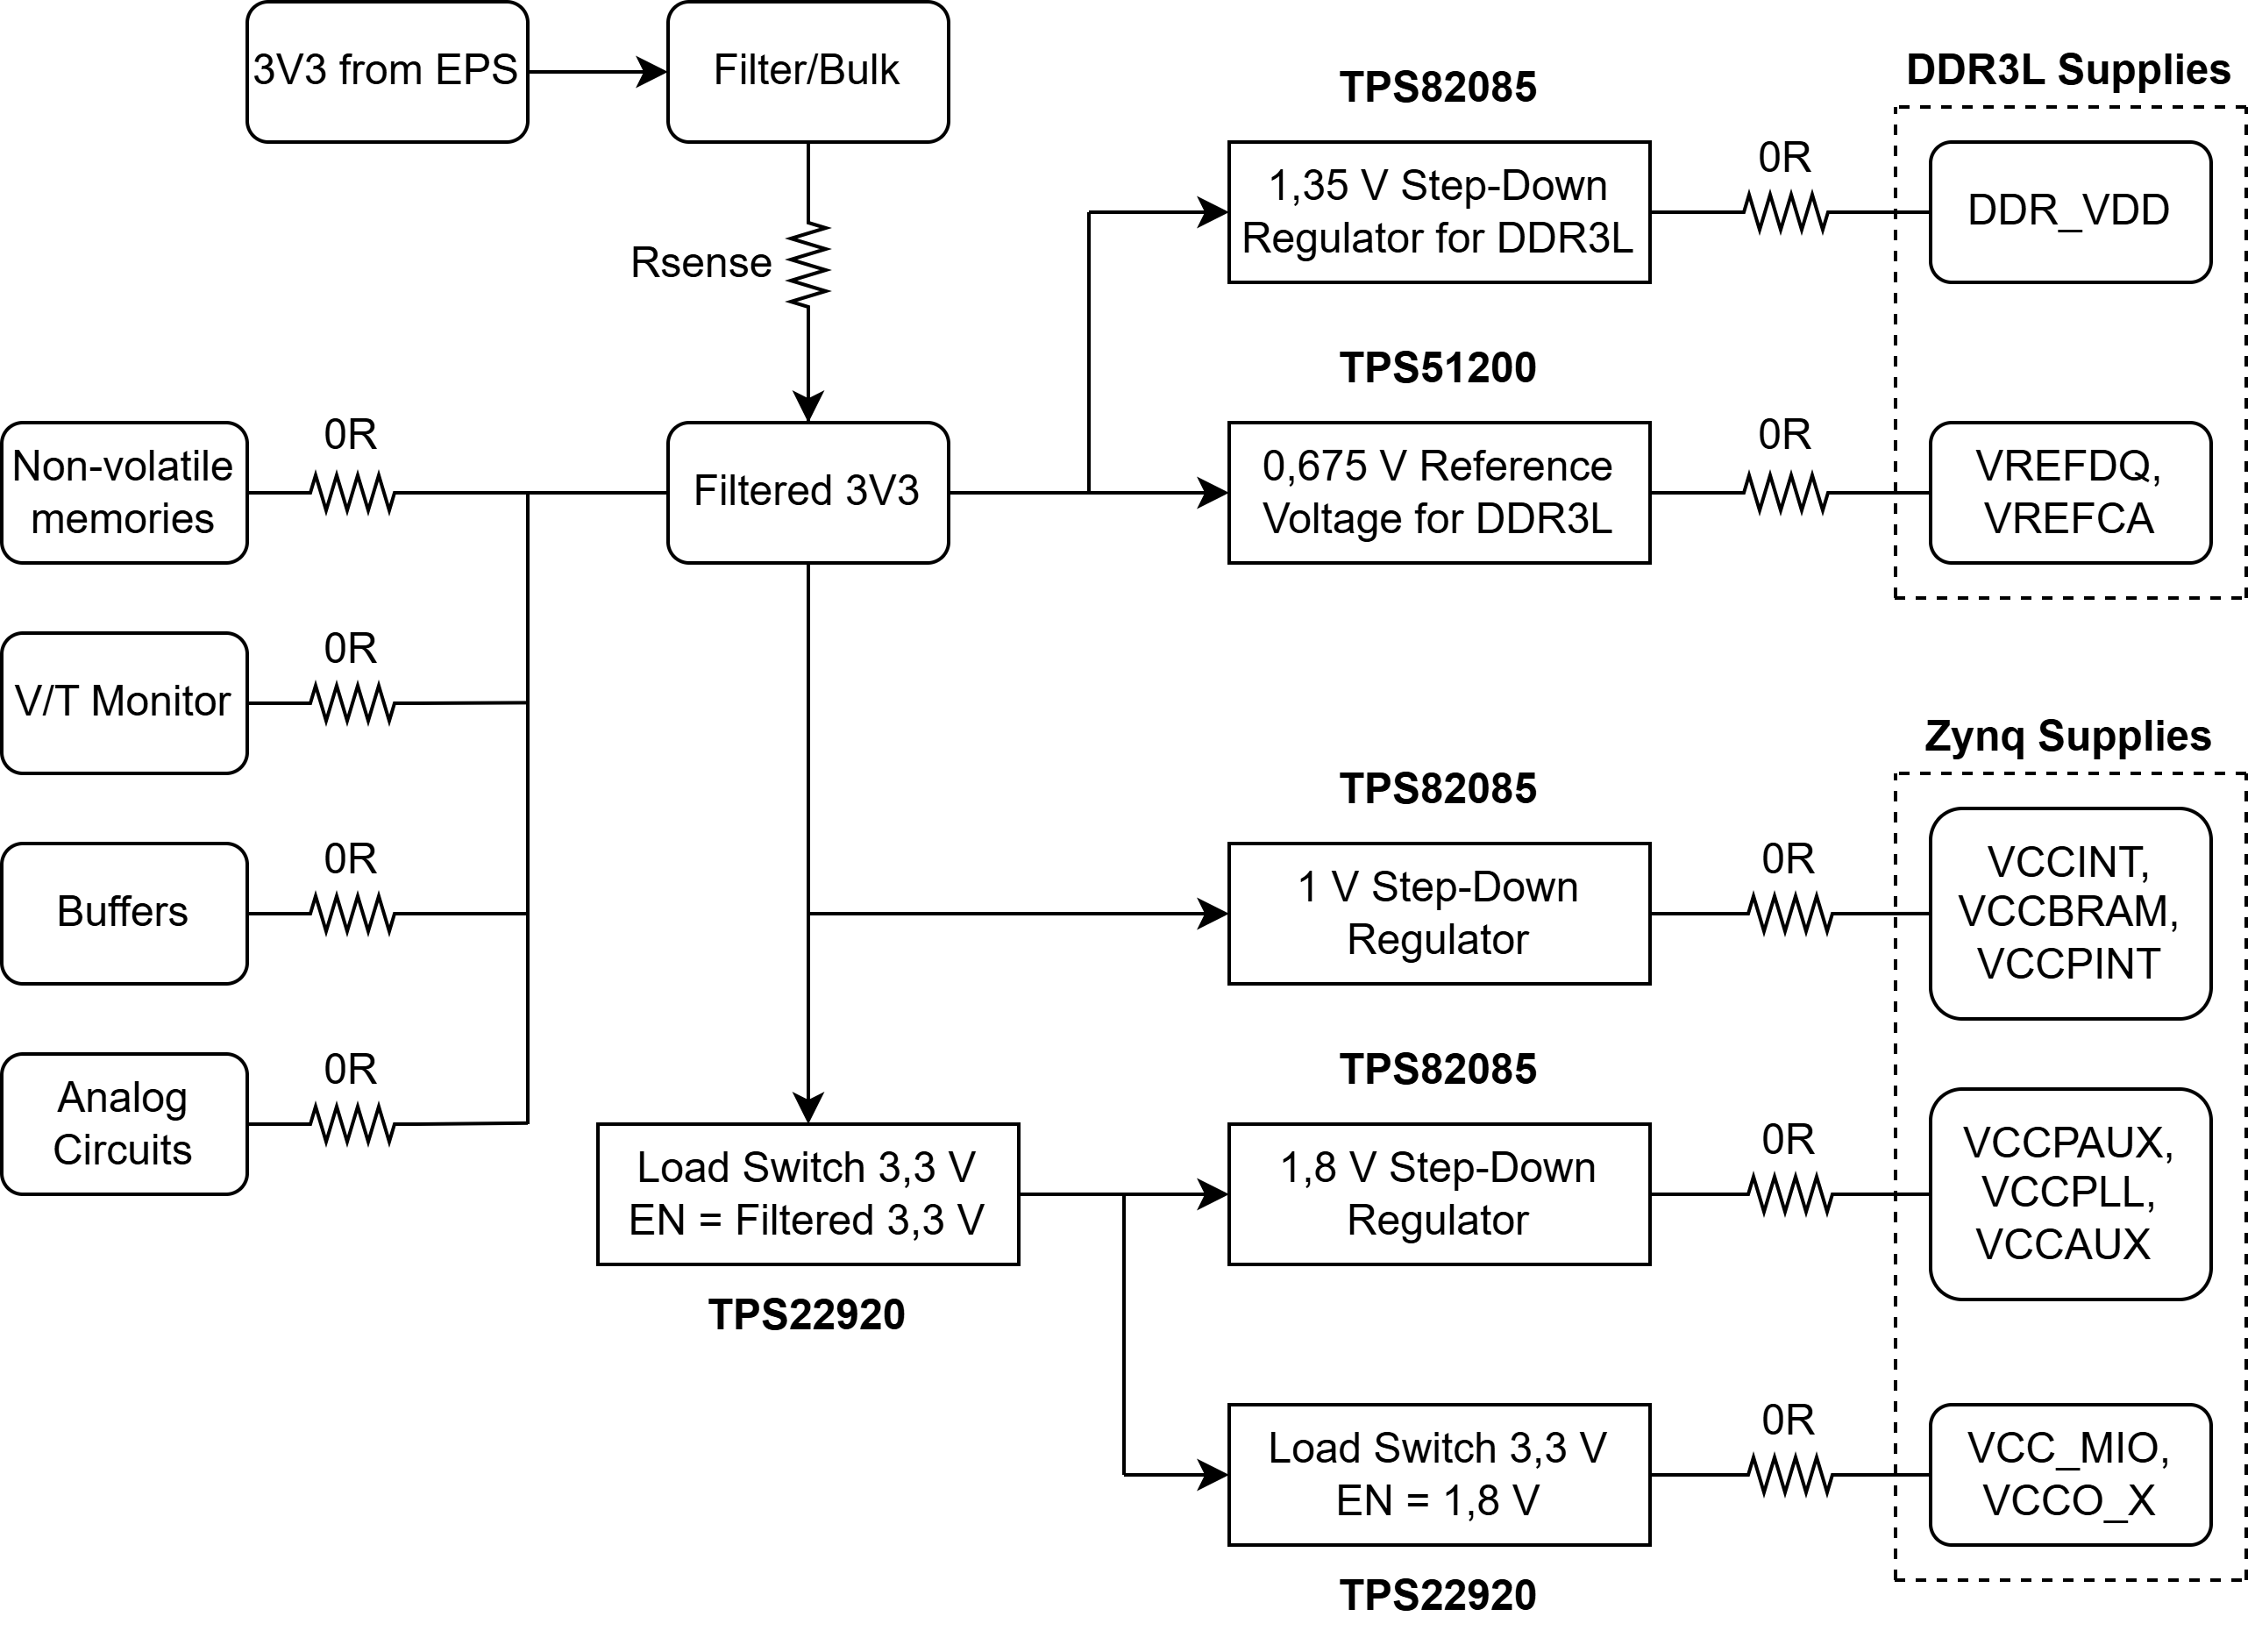
\includegraphics[scale=0.6]{images/Power_system.png}
    \caption{Cascata de potência proposta.}
    \label{fig:power}
    \fonte{Elaboração própria.}
\end{figure}

\subsection{Filtro de Entrada}

Costumeiramente, a entrada de tensão de uma placa robusta deve ser filtrada, principalmente devido às flutuações do ruído conduzido de outros subsistemas do satélite, caracterizando o fenômeno de Interferência Eletromagnética (EMI), esquematizado na Figura \ref{fig:emi}.

\begin{figure}[H]
    \centering
    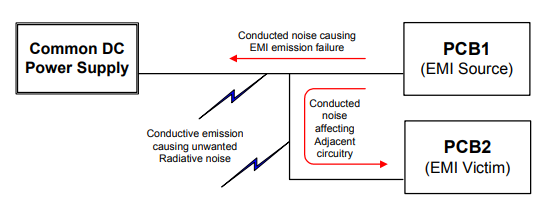
\includegraphics[scale=1]{images/EMI noise.png}
    \caption{Interferência com ruído conduzido.}
    \label{fig:emi}
    \fonte{SOH et al., 2010.}
\end{figure}

Além disso, também foi necessária a inclusão de um diodo Zener em paralelo à entrada, servindo como um elemento extra de proteção contra perturbações e transientes (CADENCE, 2023). Outra característica explorada foi a colocação de capacitores em paralelo, a fim de reduzir sua resistência em série equivalente (ESR) e sua indutância série (SARJEANT, 1990).  O filtro proposto está disposto na Figura \ref{fig:FILTRO}.  Além disso, sua magnitude e fase simuladas estão dispostas na Figura \ref{fig:filtrof}.

\begin{figure}[H]
    \centering
    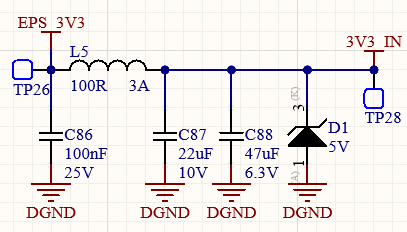
\includegraphics[scale=1]{images/FILTRO.png}
    \caption{Filtro proposto.}
    \label{fig:FILTRO}
    \fonte{Elaboração própria.}
\end{figure}

\begin{figure}[H]
    \centering
    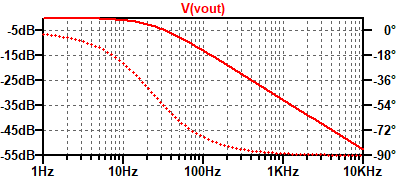
\includegraphics[scale=1]{images/filtrof.png}
    \caption{Simulação de magnitude e fase em função da frequência para o filtro proposto.}
    \label{fig:filtrof}
    \fonte{Elaboração própria.}
\end{figure}

\subsection{Cascata de potência}

Devido à escolha do SoC e da memória DDR3, foi necessária a definição de uma cascata de potência, levando-se em consideração os requisitos de (UG585, 2023), que descreve o sequenciamento das tensões para o menor consumo de potência e para garantir a integridade do fusível interno do SoC. Dessa forma, como pode-se ver na Figura \ref{fig:power}, são usados os denominados \textit{load switches}, a fim de garantir o sequenciamento descrito e garantir uma proteção efetiva contra sobrecorrente (MAK, 2018). 

O primeiro regulador, que gera a tensão de 1 V, apresentado na Figura \ref{fig:1vsupp}, é o primeiro da cascata. Seu divisor de tensão de saída foi calculado conforme (TPS82085, 2019):

\begin{equation}
	V_{out} = 0,8 * (1 + R_1/R_2) = 0,8 * (1+ 37,4k/150k) = 0,999 V
\end{equation} 

\begin{figure}[H]
    \centering
    \includegraphics[scale=0.8]{images/1vsupp.png}
    \caption{Regulador de tensão de 1 V.}
    \label{fig:1vsupp}
    \fonte{Elaboração própria com base no circuito apresentado pelo fabricante.}
\end{figure}

Também foi possível montar seu circuito de proteção de sobrecorrente, disposto na Figura \ref{fig:1vocp}. Seu resistor de entrada, que escolhe o limiar de corrente permitido, foi caculado conforme (LTC4361, 2018), considerando uma corrente 20\% superior à máxima calculada (na Tabela \ref{tab:estpow}):

\begin{equation}
	R_{sense} = 50 mV / I_{max} =50 / 2,63 = 19,01 m\Omega
\end{equation} 

\begin{figure}[H]
    \centering
    \includegraphics[scale=1]{images/1vocp.png}
    \caption{Proteção contra \textit{latch-up} para a tensão de 1 V.}
    \label{fig:1vocp}
    \fonte{Elaboração própria com base no circuito apresentado pelo fabricante.}
\end{figure}

Depois disso, para seguir com o sequenciamento requerido pelo SoC, precisa-se de um circuito de chaveamento de carga, apresentado na Figura \ref{fig:sw1}. Seu circuito é baseado no sugerido por (TPS22920, 2016), com seu ligamento sendo feito pela própria tensão de 3,3 V.

\begin{figure}[H]
    \centering
    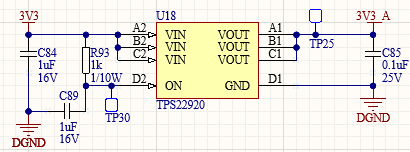
\includegraphics[scale=1]{images/sw1.png}
    \caption{Circuito de \textit{Load switch} para a tensão de 1,8 V.}
    \label{fig:sw1}
    \fonte{Elaboração própria com base no circuito apresentado pelo fabricante.}
\end{figure}

Analogamente, para a tensão de 1,8 V, são necessários ambos um conversor e um circuito de proteção. Estes estão dispostos respectivamente nas Figuras \ref{fig:1v8supp} e \ref{fig:1v8ocp} a seguir, conjuntamente com suas equações (3) e (4) para obtenção das resistências requeridas, usando a mesma margem de 20\% de corrente máxima. 

\begin{equation}
	V_{out} = 0,8 * (1 + R_1/R_2) = 0,8 * (1+ 110k/88,7k) = 1,792 V
\end{equation} 

\begin{figure}[H]
    \centering
    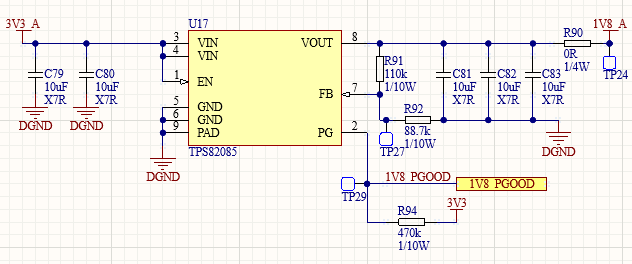
\includegraphics[scale=0.8]{images/1v8supp.png}
    \caption{Regulador de tensão de 1,8 V.}
    \label{fig:1v8supp}
    \fonte{Elaboração própria com base no circuito apresentado pelo fabricante.}
\end{figure}

\begin{equation}
	R_{sense} = 50 mV / I_{max} =50 / 0,5 = 100 m\Omega
\end{equation} 

\begin{figure}[H]
    \centering
    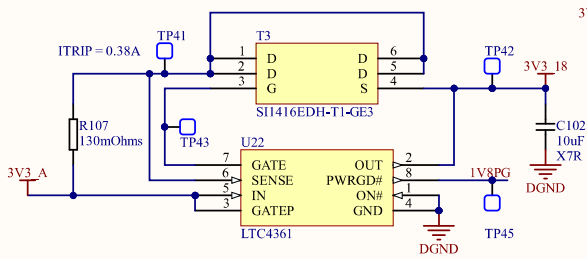
\includegraphics[scale=1]{images/1v8ocp.png}
    \caption{Proteção contra \textit{latch-up} para a tensão de 1,8 V.}
    \label{fig:1v8ocp}
    \fonte{Elaboração própria com base no circuito apresentado pelo fabricante.}
\end{figure}

Por fim, para ligar a tensão de 3,3 V fornecida para o SoC, é necessário um último circuito de chaveamento, dessa vez com seu ligamento feito pela tensão de 1,8 V, como mostra a Figura \ref{fig:sw2}.

\begin{figure}[H]
    \centering
    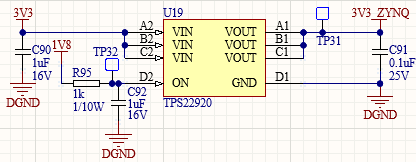
\includegraphics[scale=1]{images/sw2.png}
    \caption{Circuito de \textit{Load switch} para a tensão de 3,3 V do SoC.}
    \label{fig:sw2}
    \fonte{Elaboração própria com base no circuito apresentado pelo fabricante.}
\end{figure}

Paralelamente, para a memória DDR3L, são necessários um conversor para a alimentação, de 1,35 V, e um conversor para a tensão de referência e de terminação. Esses circuitos estão dispostos respectivamente nas Figuras \ref{fig:1v35supp} e \ref.

\begin{equation}
	V_{out} = 0,8 * (1 + R_1/R_2) = 0,8 * (1+ 47k/68k) = 1,353 V
\end{equation} 

\begin{figure}[H]
    \centering
    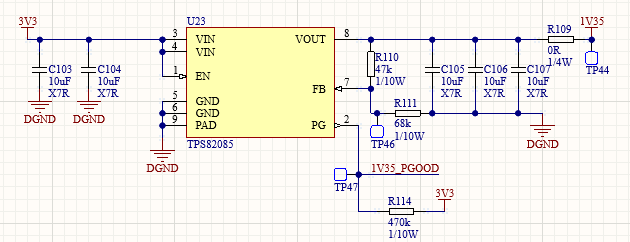
\includegraphics[scale=0.8]{images/1v35supp.png}
    \caption{Regulador de tensão de 1,35 V.}
    \label{fig:1v35supp}
    \fonte{Elaboração própria com base no circuito apresentado pelo fabricante.}
\end{figure}

\begin{figure}[H]
    \centering
    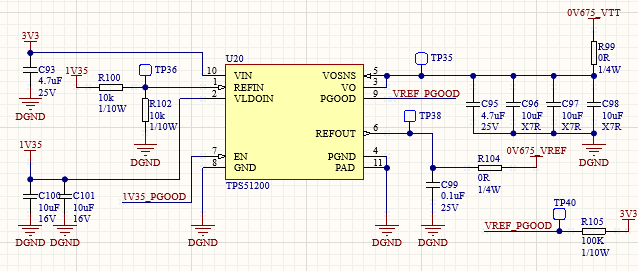
\includegraphics[scale=0.8]{images/refsupp.png}
    \caption{Regulador de tensão de referência e terminação para a memória DDR3L.}
    \label{fig:1v35ref}
    \fonte{Elaboração própria com base no circuito apresentado pelo fabricante.}
\end{figure}

\section{SoC}

No caso do SoC Zynq 7030, temos no total seis blocos operacionais, que incluem o funcionamento do PL e do PS, bem como as configurações e o bloco dedicado ao controlador da memória DDR (UG585, 2023). A seguir, estão dispostas as descrições funcionais e circuitos necessários para o funcionamento correto desse SoC, separados por bloco funcional.

\subsection{Bloco de Configuração}

\subsection{Blocos do PS}

\subsection{Blocos do PL}

\subsection{Bloco Controlador da Memória DDR}

\subsection{Pinos de Potência}

\section{Conexões entre blocos}